\INEchaptercarta{Pobreza}{}


\cajita{Línea de pobreza total}{La línea de pobreza extrema representa el costo de adquirir la cantidad mínima de calorías recomendadas.  La línea de pobreza total incluye, además del costo alimenticio, un monto adicional que corresponde al porcentaje de consumo no alimenticio de las personas cuyo consumo de alimentos se encuentra alrededor de la línea de pobreza extrema. }{Línea de pobreza total}{República de Guatemala, serie histórica por Encovi,  en quetzales corrientes}{\ \\[0mm]\begin{tikzpicture}[x=1pt,y=1pt]  % Created by tikzDevice version 0.7.0 on 2015-11-27 11:12:31
% !TEX encoding = UTF-8 Unicode
\definecolor[named]{fillColor}{rgb}{1.00,1.00,1.00}
\path[use as bounding box,fill=fillColor,fill opacity=0.00] (0,0) rectangle (289.08,198.74);
\begin{scope}
\path[clip] (  0.00,  0.00) rectangle (289.08,198.74);

\path[] (  0.00,  0.00) rectangle (289.08,198.74);
\end{scope}
\begin{scope}
\path[clip] (  0.00,  0.00) rectangle (289.08,198.74);

\path[] ( 14.78, 17.78) rectangle (280.54,191.48);

\path[] ( 14.78, 34.98) --
	(280.54, 34.98);

\path[] ( 14.78, 76.15) --
	(280.54, 76.15);

\path[] ( 14.78,117.33) --
	(280.54,117.33);

\path[] ( 14.78,158.51) --
	(280.54,158.51);

\path[] ( 14.78, 55.57) --
	(280.54, 55.57);

\path[] ( 14.78, 96.74) --
	(280.54, 96.74);

\path[] ( 14.78,137.92) --
	(280.54,137.92);

\path[] ( 14.78,179.10) --
	(280.54,179.10);

\path[] ( 64.61, 17.78) --
	( 64.61,191.48);

\path[] (147.66, 17.78) --
	(147.66,191.48);

\path[] (230.71, 17.78) --
	(230.71,191.48);
\definecolor[named]{drawColor}{rgb}{0.00,0.00,1.00}

\path[draw=drawColor,line width= 1.7pt,line join=round] ( 64.61, 62.11) --
	(147.66,108.56) --
	(230.71,183.59);
\definecolor[named]{drawColor}{rgb}{0.00,0.00,0.00}

\node[text=drawColor,anchor=base,inner sep=0pt, outer sep=0pt, scale=  1.01] at ( 64.61, 50.24) {4,318};

\node[text=drawColor,anchor=base east,inner sep=0pt, outer sep=0pt, scale=  1.01] at (143.66,108.56) {6,574};

\node[text=drawColor,anchor=base,inner sep=0pt, outer sep=0pt, scale=  1.01] at (230.71,187.54) {10,218};
\definecolor[named]{fillColor}{rgb}{0.00,0.00,0.00}

\path[draw=drawColor,line width= 0.1pt,line join=round,fill=fillColor] ( 14.78, 25.67) -- (280.54, 25.67);

\path[] ( 14.78, 17.78) rectangle (280.54,191.48);
\end{scope}
\begin{scope}
\path[clip] (  0.00,  0.00) rectangle (289.08,198.74);

\path[] ( 14.78, 17.78) --
	( 14.78,191.48);
\end{scope}
\begin{scope}
\path[clip] (  0.00,  0.00) rectangle (289.08,198.74);
\definecolor[named]{drawColor}{rgb}{1.00,1.00,1.00}

\node[text=drawColor,text opacity=0.00,anchor=base east,inner sep=0pt, outer sep=0pt, scale=  1.00] at (  7.67, 51.66) {4000};

\node[text=drawColor,text opacity=0.00,anchor=base east,inner sep=0pt, outer sep=0pt, scale=  1.00] at (  7.67, 92.84) {6000};

\node[text=drawColor,text opacity=0.00,anchor=base east,inner sep=0pt, outer sep=0pt, scale=  1.00] at (  7.67,134.01) {8000};

\node[text=drawColor,text opacity=0.00,anchor=base east,inner sep=0pt, outer sep=0pt, scale=  1.00] at (  7.67,175.19) {10000};
\end{scope}
\begin{scope}
\path[clip] (  0.00,  0.00) rectangle (289.08,198.74);

\path[] ( 10.51, 55.57) --
	( 14.78, 55.57);

\path[] ( 10.51, 96.74) --
	( 14.78, 96.74);

\path[] ( 10.51,137.92) --
	( 14.78,137.92);

\path[] ( 10.51,179.10) --
	( 14.78,179.10);
\end{scope}
\begin{scope}
\path[clip] (  0.00,  0.00) rectangle (289.08,198.74);

\path[] ( 14.78, 17.78) --
	(280.54, 17.78);
\end{scope}
\begin{scope}
\path[clip] (  0.00,  0.00) rectangle (289.08,198.74);

\path[] ( 64.61, 13.51) --
	( 64.61, 17.78);

\path[] (147.66, 13.51) --
	(147.66, 17.78);

\path[] (230.71, 13.51) --
	(230.71, 17.78);
\end{scope}
\begin{scope}
\path[clip] (  0.00,  0.00) rectangle (289.08,198.74);
\definecolor[named]{drawColor}{rgb}{0.00,0.00,0.00}

\node[text=drawColor,anchor=base,inner sep=0pt, outer sep=0pt, scale=  1.00] at ( 64.61,  2.85) {2000};

\node[text=drawColor,anchor=base,inner sep=0pt, outer sep=0pt, scale=  1.00] at (147.66,  2.85) {2006};

\node[text=drawColor,anchor=base,inner sep=0pt, outer sep=0pt, scale=  1.00] at (230.71,  2.85) {2014};
\end{scope}
  \end{tikzpicture}}{Instituto Nacional de Estadística}


\cajita{Pobreza total}{\footnote{$FGT(\alpha)=$
		
		$ \frac{1}{N}\sum_{i=1}^N \left(1-\frac{x_i}{LPT}\right)^\alpha (x_i<LPT) $\\
		
		Con $\alpha=0$}  Para 2014, el \% de la población se encontraba por debajo de la línea de pobreza total y el \% no lograba cubrir el costo del consumo mínimo de alimentos. Se puede observar en la gráfica  que entre 2000 y 2014, la pobreza extrema se redujo / aumentó en x puntos porcentuales, pasando de 15.7\% en 2000 a \% en 2014, mientras que la pobreza total de 56.4\% a \%.  }{Incidencia de pobreza total }{República de Guatemala, serie histórica por Encovi,  en porcentaje}{\ \\[0mm]\begin{tikzpicture}[x=1pt,y=1pt]  % Created by tikzDevice version 0.7.0 on 2015-11-27 11:12:32
% !TEX encoding = UTF-8 Unicode
\definecolor[named]{fillColor}{rgb}{1.00,1.00,1.00}
\path[use as bounding box,fill=fillColor,fill opacity=0.00] (0,0) rectangle (289.08,198.74);
\begin{scope}
\path[clip] (  0.00,  0.00) rectangle (289.08,198.74);

\path[] (  0.00,  0.00) rectangle (289.08,198.74);
\end{scope}
\begin{scope}
\path[clip] (  0.00,  0.00) rectangle (289.08,198.74);

\path[] (  1.64, 17.78) rectangle (280.54,191.48);

\path[] (  1.64, 37.36) --
	(280.54, 37.36);

\path[] (  1.64, 82.20) --
	(280.54, 82.20);

\path[] (  1.64,127.03) --
	(280.54,127.03);

\path[] (  1.64,171.86) --
	(280.54,171.86);

\path[] (  1.64, 59.78) --
	(280.54, 59.78);

\path[] (  1.64,104.61) --
	(280.54,104.61);

\path[] (  1.64,149.44) --
	(280.54,149.44);

\path[] ( 53.94, 17.78) --
	( 53.94,191.48);

\path[] (141.09, 17.78) --
	(141.09,191.48);

\path[] (228.25, 17.78) --
	(228.25,191.48);
\definecolor[named]{drawColor}{rgb}{0.00,0.00,1.00}

\path[draw=drawColor,line width= 1.7pt,line join=round] ( 53.94,140.63) --
	(141.09, 62.11) --
	(228.25,183.59);
\definecolor[named]{drawColor}{rgb}{0.00,0.00,0.00}

\node[text=drawColor,anchor=base,inner sep=0pt, outer sep=0pt, scale=  1.01] at ( 53.94,144.58) {56.4};

\node[text=drawColor,anchor=base,inner sep=0pt, outer sep=0pt, scale=  1.01] at (141.09, 50.24) {51.2};

\node[text=drawColor,anchor=base,inner sep=0pt, outer sep=0pt, scale=  1.01] at (228.25,187.54) {59.3};
\definecolor[named]{fillColor}{rgb}{0.00,0.00,0.00}

\path[draw=drawColor,line width= 0.1pt,line join=round,fill=fillColor] (  1.64, 25.67) -- (280.54, 25.67);

\path[] (  1.64, 17.78) rectangle (280.54,191.48);
\end{scope}
\begin{scope}
\path[clip] (  0.00,  0.00) rectangle (289.08,198.74);

\path[] (  1.64, 17.78) --
	(  1.64,191.48);
\end{scope}
\begin{scope}
\path[clip] (  0.00,  0.00) rectangle (289.08,198.74);

\path[] (  0.00, 59.78) --
	(  1.64, 59.78);

\path[] (  0.00,104.61) --
	(  1.64,104.61);

\path[] (  0.00,149.44) --
	(  1.64,149.44);
\end{scope}
\begin{scope}
\path[clip] (  0.00,  0.00) rectangle (289.08,198.74);

\path[] (  1.64, 17.78) --
	(280.54, 17.78);
\end{scope}
\begin{scope}
\path[clip] (  0.00,  0.00) rectangle (289.08,198.74);

\path[] ( 53.94, 13.51) --
	( 53.94, 17.78);

\path[] (141.09, 13.51) --
	(141.09, 17.78);

\path[] (228.25, 13.51) --
	(228.25, 17.78);
\end{scope}
\begin{scope}
\path[clip] (  0.00,  0.00) rectangle (289.08,198.74);
\definecolor[named]{drawColor}{rgb}{0.00,0.00,0.00}

\node[text=drawColor,anchor=base,inner sep=0pt, outer sep=0pt, scale=  1.00] at ( 53.94,  2.85) {2000};

\node[text=drawColor,anchor=base,inner sep=0pt, outer sep=0pt, scale=  1.00] at (141.09,  2.85) {2006};

\node[text=drawColor,anchor=base,inner sep=0pt, outer sep=0pt, scale=  1.00] at (228.25,  2.85) {2014};
\end{scope}
  \end{tikzpicture}}{Instituto Nacional de Estadística}


\cajita{Pobreza total por área de residencia}{\textollamada{Para el año 2014, el X\% de la población habitaba en áreas urbanas y el y\% en áreas rurales.} Al desagregar por las distintas características de la población, se observan amplias brechas entre los distintos grupos de población. En general, los mayores niveles de pobreza se observan en la población indígena y la población que habita en áreas rurales. Aunque la pobreza se ha reducido para estos dos grupos de población en el período estudiado, las diferencias todavía son amplias con relación a la población no indígena y a la población que habita  en áreas urbanas, respectivamente. }{Incidencia de pobreza total por área de residencia}{República de Guatemala, serie histórica por Encovi,  en porcentaje}{\ \\[0mm]\begin{tikzpicture}[x=1pt,y=1pt]  % Created by tikzDevice version 0.9 on 2015-12-01 14:57:19
% !TEX encoding = UTF-8 Unicode
\definecolor{fillColor}{RGB}{255,255,255}
\path[use as bounding box,fill=fillColor,fill opacity=0.00] (0,0) rectangle (289.08,198.74);
\begin{scope}
\path[clip] (  0.00,  0.00) rectangle (289.08,198.74);

\path[] (  0.00,  0.00) rectangle (289.08,198.74);
\end{scope}
\begin{scope}
\path[clip] (  0.00,  0.00) rectangle (289.08,198.74);

\path[] (  7.11, 20.62) rectangle (289.08,172.42);

\path[] ( 59.98, 20.62) --
	( 59.98,172.42);

\path[] (148.10, 20.62) --
	(148.10,172.42);

\path[] (236.21, 20.62) --
	(236.21,172.42);
\definecolor{drawColor}{RGB}{0,0,255}
\definecolor{fillColor}{RGB}{0,0,255}

\path[draw=drawColor,line width= 0.6pt,line join=round,fill=fillColor] ( 26.94, 20.62) rectangle ( 53.37,168.70);
\definecolor{drawColor}{RGB}{157,187,255}
\definecolor{fillColor}{RGB}{157,187,255}

\path[draw=drawColor,line width= 0.6pt,line join=round,fill=fillColor] ( 66.59, 20.62) rectangle ( 93.02,100.90);
\definecolor{drawColor}{RGB}{0,0,255}
\definecolor{fillColor}{RGB}{0,0,255}

\path[draw=drawColor,line width= 0.6pt,line join=round,fill=fillColor] (115.05, 20.62) rectangle (141.49,164.31);
\definecolor{drawColor}{RGB}{157,187,255}
\definecolor{fillColor}{RGB}{157,187,255}

\path[draw=drawColor,line width= 0.6pt,line join=round,fill=fillColor] (154.71, 20.62) rectangle (181.14, 90.23);
\definecolor{drawColor}{RGB}{0,0,255}
\definecolor{fillColor}{RGB}{0,0,255}

\path[draw=drawColor,line width= 0.6pt,line join=round,fill=fillColor] (203.17, 20.62) rectangle (229.60,172.42);
\definecolor{drawColor}{RGB}{157,187,255}
\definecolor{fillColor}{RGB}{157,187,255}

\path[draw=drawColor,line width= 0.6pt,line join=round,fill=fillColor] (242.82, 20.62) rectangle (269.25,109.86);
\definecolor{drawColor}{RGB}{0,0,0}

\path[draw=drawColor,line width= 0.6pt,line join=round] (  7.11, 20.62) -- (289.08, 20.62);

\node[text=drawColor,anchor=base,inner sep=0pt, outer sep=0pt, scale=  0.82] at ( 40.16,171.92) {77.3};

\node[text=drawColor,anchor=base,inner sep=0pt, outer sep=0pt, scale=  0.82] at ( 79.81,104.13) {41.9};

\node[text=drawColor,anchor=base,inner sep=0pt, outer sep=0pt, scale=  0.82] at (128.27,167.53) {75.0};

\node[text=drawColor,anchor=base,inner sep=0pt, outer sep=0pt, scale=  0.82] at (167.92, 93.45) {36.3};

\node[text=drawColor,anchor=base,inner sep=0pt, outer sep=0pt, scale=  0.82] at (216.39,175.65) {79.2};

\node[text=drawColor,anchor=base,inner sep=0pt, outer sep=0pt, scale=  0.82] at (256.04,113.08) {46.6};

\path[] (  7.11, 20.62) rectangle (289.08,172.42);
\end{scope}
\begin{scope}
\path[clip] (  0.00,  0.00) rectangle (289.08,198.74);

\path[] (  7.11, 20.62) --
	(  7.11,172.42);
\end{scope}
\begin{scope}
\path[clip] (  0.00,  0.00) rectangle (289.08,198.74);

\path[] (  7.11, 20.62) --
	(289.08, 20.62);
\end{scope}
\begin{scope}
\path[clip] (  0.00,  0.00) rectangle (289.08,198.74);

\path[] ( 59.98, 16.35) --
	( 59.98, 20.62);

\path[] (148.10, 16.35) --
	(148.10, 20.62);

\path[] (236.21, 16.35) --
	(236.21, 20.62);
\end{scope}
\begin{scope}
\path[clip] (  0.00,  0.00) rectangle (289.08,198.74);
\definecolor{drawColor}{RGB}{0,0,0}

\node[text=drawColor,anchor=base,inner sep=0pt, outer sep=0pt, scale=  1.00] at ( 59.98,  5.69) {2000};

\node[text=drawColor,anchor=base,inner sep=0pt, outer sep=0pt, scale=  1.00] at (148.10,  5.69) {2006};

\node[text=drawColor,anchor=base,inner sep=0pt, outer sep=0pt, scale=  1.00] at (236.21,  5.69) {2014};
\end{scope}
\begin{scope}
\path[clip] (  0.00,  0.00) rectangle (289.08,198.74);
\coordinate (apoyo) at (55.19,188.79);
\coordinate (longitudFicticia) at (7.11,9.95);
\coordinate (longitud) at (7.11,7.11);
\coordinate (desX) at (133.24,0);
\coordinate (desY) at (0,1.42);
\definecolor[named]{ct1}{HTML}{
0000FF
}
\definecolor[named]{ct2}{HTML}{
9DBBFF
}
\definecolor[named]{ctb1}{HTML}{
0000FF
}
\definecolor[named]{ctb2}{HTML}{
9DBBFF
}
\path [fill=none] (apoyo) rectangle ($(apoyo)+(longitudFicticia)$)
node [xshift=0.3cm,inner sep=0pt, outer sep=0pt,midway,right,scale = 0.9]{Indígena};
\draw [color = ctb1,fill=ct1] ( $(apoyo)  + (desY) $) rectangle ($(apoyo)+ (desY) +(longitud)$);
\path [fill=none] ($(apoyo)+(desX)$) rectangle ($(apoyo)+(desX)+(longitudFicticia)$)
node [xshift=0.3cm,inner sep=0pt, outer sep=0pt,midway,right,scale = 0.9]{No indígena};
\draw [color = ctb2 ,fill=ct2] ( $(apoyo)  + (desY) + (desX) $) rectangle ($(apoyo)+ (desY)+ (desX) +(longitud)$);
\end{scope}
  \end{tikzpicture}}{Instituto Nacional de Estadística}


\cajita{Pobreza total por etnicidad}{\textollamada{Para el año 2014, el X\% de la población se autoidentificó como perteneciente a un pueblo indígena.} Al desagregar por las distintas características de la población, se observan amplias brechas entre los distintos grupos de población. En general, los mayores niveles de pobreza se observan en la población indígena y la población que habita en áreas rurales. Aunque la pobreza se ha reducido para estos dos grupos de población en el período estudiado, las diferencias todavía son amplias con relación a la población no indígena y a la población que habita  en áreas urbanas, respectivamente.}{Incidencia de pobreza total por etnicidad}{República de Guatemala, serie histórica por Encovi,  en porcentaje}{\ \\[0mm]\begin{tikzpicture}[x=1pt,y=1pt]  % Created by tikzDevice version 0.9 on 2015-11-26 21:53:05
% !TEX encoding = UTF-8 Unicode
\definecolor{fillColor}{RGB}{255,255,255}
\path[use as bounding box,fill=fillColor,fill opacity=0.00] (0,0) rectangle (289.08,198.74);
\begin{scope}
\path[clip] (  0.00,  0.00) rectangle (289.08,198.74);

\path[] (  0.00,  0.00) rectangle (289.08,198.74);
\end{scope}
\begin{scope}
\path[clip] (  0.00,  0.00) rectangle (289.08,198.74);

\path[] (  7.11, 20.62) rectangle (289.08,172.42);

\path[] ( 47.39, 20.62) --
	( 47.39,172.42);

\path[] (114.53, 20.62) --
	(114.53,172.42);

\path[] (181.66, 20.62) --
	(181.66,172.42);

\path[] (248.80, 20.62) --
	(248.80,172.42);
\definecolor{drawColor}{RGB}{0,0,255}
\definecolor{fillColor}{RGB}{0,0,255}

\path[draw=drawColor,line width= 0.6pt,line join=round,fill=fillColor] ( 18.86, 20.62) rectangle ( 45.72,172.42);
\definecolor{drawColor}{RGB}{157,187,255}
\definecolor{fillColor}{RGB}{157,187,255}

\path[draw=drawColor,line width= 0.6pt,line join=round,fill=fillColor] ( 49.07, 20.62) rectangle ( 75.93,102.92);
\definecolor{drawColor}{RGB}{0,0,255}
\definecolor{fillColor}{RGB}{0,0,255}

\path[draw=drawColor,line width= 0.6pt,line join=round,fill=fillColor] ( 86.00, 20.62) rectangle (112.85,167.92);
\definecolor{drawColor}{RGB}{157,187,255}
\definecolor{fillColor}{RGB}{157,187,255}

\path[draw=drawColor,line width= 0.6pt,line join=round,fill=fillColor] (116.21, 20.62) rectangle (143.06, 91.98);
\definecolor{drawColor}{RGB}{0,0,255}
\definecolor{fillColor}{RGB}{0,0,255}

\path[draw=drawColor,line width= 0.6pt,line join=round,fill=fillColor] (153.13, 20.62) rectangle (179.99,164.83);
\definecolor{drawColor}{RGB}{157,187,255}
\definecolor{fillColor}{RGB}{157,187,255}

\path[draw=drawColor,line width= 0.6pt,line join=round,fill=fillColor] (183.34, 20.62) rectangle (210.20,100.35);
\definecolor{drawColor}{RGB}{0,0,255}
\definecolor{fillColor}{RGB}{0,0,255}

\path[draw=drawColor,line width= 0.6pt,line join=round,fill=fillColor] (220.27, 20.62) rectangle (247.12, 20.62);
\definecolor{drawColor}{RGB}{157,187,255}
\definecolor{fillColor}{RGB}{157,187,255}

\path[draw=drawColor,line width= 0.6pt,line join=round,fill=fillColor] (250.48, 20.62) rectangle (277.33, 20.62);
\definecolor{drawColor}{RGB}{0,0,0}

\path[draw=drawColor,line width= 0.6pt,line join=round] (  7.11, 20.62) -- (289.08, 20.62);

\node[text=drawColor,anchor=base,inner sep=0pt, outer sep=0pt, scale=  0.82] at ( 32.29,175.65) {77.3};

\node[text=drawColor,anchor=base,inner sep=0pt, outer sep=0pt, scale=  0.82] at ( 62.50,106.15) {41.9};

\node[text=drawColor,anchor=base,inner sep=0pt, outer sep=0pt, scale=  0.82] at ( 99.42,171.15) {75.0};

\node[text=drawColor,anchor=base,inner sep=0pt, outer sep=0pt, scale=  0.82] at (129.63, 95.20) {36.3};

\node[text=drawColor,anchor=base,inner sep=0pt, outer sep=0pt, scale=  0.82] at (166.56,168.05) {73.4};

\node[text=drawColor,anchor=base,inner sep=0pt, outer sep=0pt, scale=  0.82] at (196.77,103.57) {40.6};

\node[text=drawColor,anchor=base,inner sep=0pt, outer sep=0pt, scale=  0.82] at (233.69, 23.84) {0.0};

\node[text=drawColor,anchor=base,inner sep=0pt, outer sep=0pt, scale=  0.82] at (263.90, 23.84) {0.0};

\path[] (  7.11, 20.62) rectangle (289.08,172.42);
\end{scope}
\begin{scope}
\path[clip] (  0.00,  0.00) rectangle (289.08,198.74);

\path[] (  7.11, 20.62) --
	(  7.11,172.42);
\end{scope}
\begin{scope}
\path[clip] (  0.00,  0.00) rectangle (289.08,198.74);

\path[] (  7.11, 20.62) --
	(289.08, 20.62);
\end{scope}
\begin{scope}
\path[clip] (  0.00,  0.00) rectangle (289.08,198.74);

\path[] ( 47.39, 16.35) --
	( 47.39, 20.62);

\path[] (114.53, 16.35) --
	(114.53, 20.62);

\path[] (181.66, 16.35) --
	(181.66, 20.62);

\path[] (248.80, 16.35) --
	(248.80, 20.62);
\end{scope}
\begin{scope}
\path[clip] (  0.00,  0.00) rectangle (289.08,198.74);
\definecolor{drawColor}{RGB}{0,0,0}

\node[text=drawColor,anchor=base,inner sep=0pt, outer sep=0pt, scale=  1.00] at ( 47.39,  5.69) {2000};

\node[text=drawColor,anchor=base,inner sep=0pt, outer sep=0pt, scale=  1.00] at (114.53,  5.69) {2006};

\node[text=drawColor,anchor=base,inner sep=0pt, outer sep=0pt, scale=  1.00] at (181.66,  5.69) {2011};

\node[text=drawColor,anchor=base,inner sep=0pt, outer sep=0pt, scale=  1.00] at (248.80,  5.69) {2014};
\end{scope}
\begin{scope}
\path[clip] (  0.00,  0.00) rectangle (289.08,198.74);
\coordinate (apoyo) at (55.19,188.79);
\coordinate (longitudFicticia) at (7.11,9.95);
\coordinate (longitud) at (7.11,7.11);
\coordinate (desX) at (133.24,0);
\coordinate (desY) at (0,1.42);
\definecolor[named]{ct1}{HTML}{
0000FF
}
\definecolor[named]{ct2}{HTML}{
9DBBFF
}
\definecolor[named]{ctb1}{HTML}{
0000FF
}
\definecolor[named]{ctb2}{HTML}{
9DBBFF
}
\path [fill=none] (apoyo) rectangle ($(apoyo)+(longitudFicticia)$)
node [xshift=0.3cm,inner sep=0pt, outer sep=0pt,midway,right,scale = 0.9]{Indígena};
\draw [color = ctb1,fill=ct1] ( $(apoyo)  + (desY) $) rectangle ($(apoyo)+ (desY) +(longitud)$);
\path [fill=none] ($(apoyo)+(desX)$) rectangle ($(apoyo)+(desX)+(longitudFicticia)$)
node [xshift=0.3cm,inner sep=0pt, outer sep=0pt,midway,right,scale = 0.9]{No indígena};
\draw [color = ctb2 ,fill=ct2] ( $(apoyo)  + (desY) + (desX) $) rectangle ($(apoyo)+ (desY)+ (desX) +(longitud)$);
\end{scope}
  \end{tikzpicture}}{Instituto Nacional de Estadística}


\cajota{Pobreza total en los departamentos}{En el mapa se observa que los departamentos con mayores niveles de pobreza }{Incidencia de pobreza total}{Por departamento, año 2014, en porcentaje}{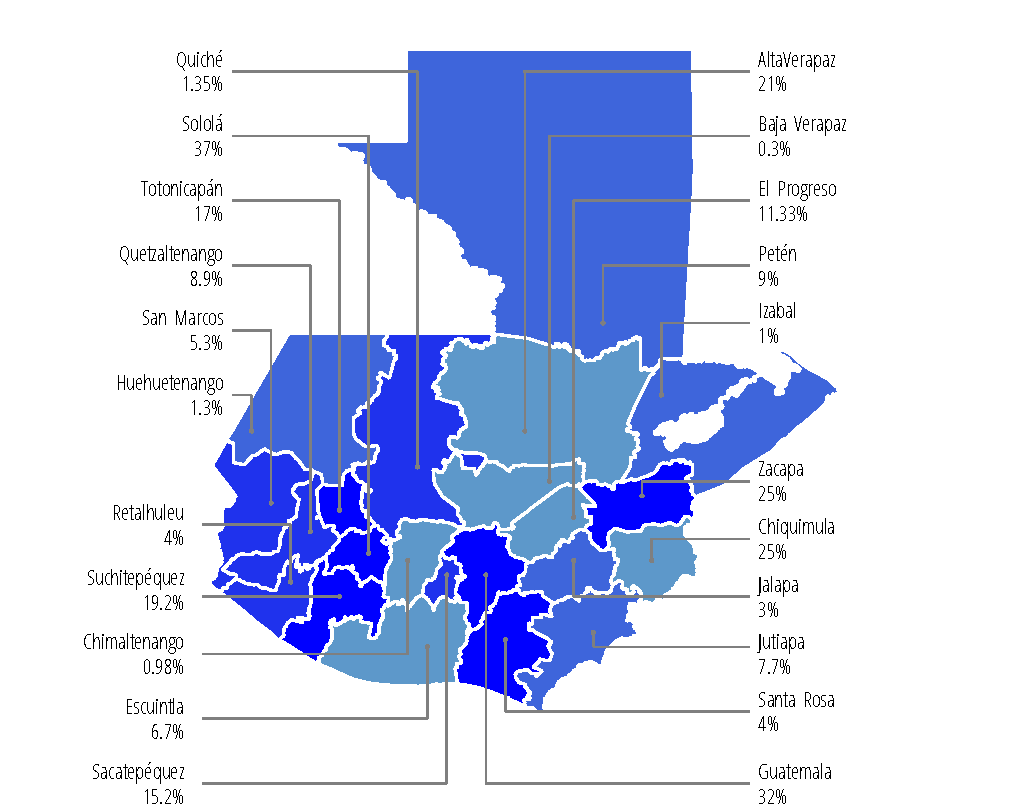
\includegraphics[width=52\cuadri]{graficas/1_05.pdf}}{Instituto Nacional de Estadística}


\cajita{Línea de pobreza extrema}{\textollamada{Para el año 2014, la cantidad de calorías mínimas recomendadas por persona al día era de. } La línea de pobreza extrema representa el costo de adquirir la cantidad mínima de calorías recomendadas.  La línea de pobreza total incluye, además del costo alimenticio, un monto adicional que corresponde al porcentaje de consumo no alimenticio de las personas cuyo consumo de alimentos se encuentra alrededor de la línea de pobreza extrema. }{Línea de pobreza extrema}{República de Guatemala, serie histórica por Encovi, en quetzales corrientes}{\ \\[0mm]\begin{tikzpicture}[x=1pt,y=1pt]  % Created by tikzDevice version 0.9 on 2015-11-26 22:12:55
% !TEX encoding = UTF-8 Unicode
\definecolor{fillColor}{RGB}{255,255,255}
\path[use as bounding box,fill=fillColor,fill opacity=0.00] (0,0) rectangle (289.08,198.74);
\begin{scope}
\path[clip] (  0.00,  0.00) rectangle (289.08,198.74);

\path[] (  0.00,  0.00) rectangle (289.08,198.74);
\end{scope}
\begin{scope}
\path[clip] (  0.00,  0.00) rectangle (289.08,198.74);

\path[] ( 10.40, 17.78) rectangle (280.54,191.48);

\path[] ( 10.40, 49.11) --
	(280.54, 49.11);

\path[] ( 10.40, 80.75) --
	(280.54, 80.75);

\path[] ( 10.40,112.39) --
	(280.54,112.39);

\path[] ( 10.40,144.03) --
	(280.54,144.03);

\path[] ( 10.40,175.68) --
	(280.54,175.68);

\path[] ( 10.40, 33.29) --
	(280.54, 33.29);

\path[] ( 10.40, 64.93) --
	(280.54, 64.93);

\path[] ( 10.40, 96.57) --
	(280.54, 96.57);

\path[] ( 10.40,128.21) --
	(280.54,128.21);

\path[] ( 10.40,159.86) --
	(280.54,159.86);

\path[] ( 61.05, 17.78) --
	( 61.05,191.48);

\path[] (145.47, 17.78) --
	(145.47,191.48);

\path[] (229.89, 17.78) --
	(229.89,191.48);
\definecolor{drawColor}{RGB}{0,0,255}

\path[draw=drawColor,line width= 1.7pt,line join=round] ( 61.05, 62.11) --
	(145.47,103.09) --
	(229.89,183.59);
\definecolor{drawColor}{RGB}{0,0,0}

\node[text=drawColor,anchor=base,inner sep=0pt, outer sep=0pt, scale=  1.01] at ( 61.05, 50.24) {1,911};

\node[text=drawColor,anchor=base east,inner sep=0pt, outer sep=0pt, scale=  1.01] at (141.47,103.09) {3,206};

\node[text=drawColor,anchor=base,inner sep=0pt, outer sep=0pt, scale=  1.01] at (229.89,187.54) {5,750};

\path[draw=drawColor,line width= 0.1pt,line join=round] ( 10.40, 25.67) -- (280.54, 25.67);

\path[] ( 10.40, 17.78) rectangle (280.54,191.48);
\end{scope}
\begin{scope}
\path[clip] (  0.00,  0.00) rectangle (289.08,198.74);

\path[] ( 10.40, 17.78) --
	( 10.40,191.48);
\end{scope}
\begin{scope}
\path[clip] (  0.00,  0.00) rectangle (289.08,198.74);
\definecolor{drawColor}{RGB}{255,255,255}

\node[text=drawColor,text opacity=0.00,anchor=base east,inner sep=0pt, outer sep=0pt, scale=  1.00] at (  3.29, 29.38) {1000};

\node[text=drawColor,text opacity=0.00,anchor=base east,inner sep=0pt, outer sep=0pt, scale=  1.00] at (  3.29, 61.02) {2000};

\node[text=drawColor,text opacity=0.00,anchor=base east,inner sep=0pt, outer sep=0pt, scale=  1.00] at (  3.29, 92.66) {3000};

\node[text=drawColor,text opacity=0.00,anchor=base east,inner sep=0pt, outer sep=0pt, scale=  1.00] at (  3.29,124.31) {4000};

\node[text=drawColor,text opacity=0.00,anchor=base east,inner sep=0pt, outer sep=0pt, scale=  1.00] at (  3.29,155.95) {5000};
\end{scope}
\begin{scope}
\path[clip] (  0.00,  0.00) rectangle (289.08,198.74);

\path[] (  6.13, 33.29) --
	( 10.40, 33.29);

\path[] (  6.13, 64.93) --
	( 10.40, 64.93);

\path[] (  6.13, 96.57) --
	( 10.40, 96.57);

\path[] (  6.13,128.21) --
	( 10.40,128.21);

\path[] (  6.13,159.86) --
	( 10.40,159.86);
\end{scope}
\begin{scope}
\path[clip] (  0.00,  0.00) rectangle (289.08,198.74);

\path[] ( 10.40, 17.78) --
	(280.54, 17.78);
\end{scope}
\begin{scope}
\path[clip] (  0.00,  0.00) rectangle (289.08,198.74);

\path[] ( 61.05, 13.51) --
	( 61.05, 17.78);

\path[] (145.47, 13.51) --
	(145.47, 17.78);

\path[] (229.89, 13.51) --
	(229.89, 17.78);
\end{scope}
\begin{scope}
\path[clip] (  0.00,  0.00) rectangle (289.08,198.74);
\definecolor{drawColor}{RGB}{0,0,0}

\node[text=drawColor,anchor=base,inner sep=0pt, outer sep=0pt, scale=  1.00] at ( 61.05,  2.85) {2000};

\node[text=drawColor,anchor=base,inner sep=0pt, outer sep=0pt, scale=  1.00] at (145.47,  2.85) {2006};

\node[text=drawColor,anchor=base,inner sep=0pt, outer sep=0pt, scale=  1.00] at (229.89,  2.85) {2014};
\end{scope}
  \end{tikzpicture}}{Instituto Nacional de Estadística}


\cajita{Pobreza extrema}{\footnote{$FGT(\alpha)=$
		
		$ \frac{1}{N}\sum_{i=1}^N \left(1-\frac{x_i}{LPT}\right)^\alpha (x_i<LPT) $\\
		
		Con $\alpha=0$} }{Incidencia de pobreza extrema}{República de Guatemala, serie histórica por Encovi, en porcentaje}{\ \\[0mm]\begin{tikzpicture}[x=1pt,y=1pt]  % Created by tikzDevice version 0.9 on 2015-11-26 22:17:03
% !TEX encoding = UTF-8 Unicode
\definecolor{fillColor}{RGB}{255,255,255}
\path[use as bounding box,fill=fillColor,fill opacity=0.00] (0,0) rectangle (289.08,198.74);
\begin{scope}
\path[clip] (  0.00,  0.00) rectangle (289.08,198.74);

\path[] (  0.00,  0.00) rectangle (289.08,198.74);
\end{scope}
\begin{scope}
\path[clip] (  0.00,  0.00) rectangle (289.08,198.74);

\path[] (  1.64, 17.78) rectangle (280.54,191.48);

\path[] (  1.64, 35.67) --
	(280.54, 35.67);

\path[] (  1.64, 80.69) --
	(280.54, 80.69);

\path[] (  1.64,125.72) --
	(280.54,125.72);

\path[] (  1.64,170.74) --
	(280.54,170.74);

\path[] (  1.64, 58.18) --
	(280.54, 58.18);

\path[] (  1.64,103.21) --
	(280.54,103.21);

\path[] (  1.64,148.23) --
	(280.54,148.23);

\path[] ( 53.94, 17.78) --
	( 53.94,191.48);

\path[] (141.09, 17.78) --
	(141.09,191.48);

\path[] (228.25, 17.78) --
	(228.25,191.48);
\definecolor{drawColor}{RGB}{0,0,255}

\path[draw=drawColor,line width= 1.7pt,line join=round] ( 53.94, 68.69) --
	(141.09, 62.11) --
	(228.25,183.59);
\definecolor{drawColor}{RGB}{0,0,0}

\node[text=drawColor,anchor=base,inner sep=0pt, outer sep=0pt, scale=  1.01] at ( 53.94, 72.64) {15.7};

\node[text=drawColor,anchor=base,inner sep=0pt, outer sep=0pt, scale=  1.01] at (141.09, 50.24) {15.3};

\node[text=drawColor,anchor=base,inner sep=0pt, outer sep=0pt, scale=  1.01] at (228.25,187.54) {23.4};

\path[draw=drawColor,line width= 0.1pt,line join=round] (  1.64, 25.67) -- (280.54, 25.67);

\path[] (  1.64, 17.78) rectangle (280.54,191.48);
\end{scope}
\begin{scope}
\path[clip] (  0.00,  0.00) rectangle (289.08,198.74);

\path[] (  1.64, 17.78) --
	(  1.64,191.48);
\end{scope}
\begin{scope}
\path[clip] (  0.00,  0.00) rectangle (289.08,198.74);

\path[] (  0.00, 58.18) --
	(  1.64, 58.18);

\path[] (  0.00,103.21) --
	(  1.64,103.21);

\path[] (  0.00,148.23) --
	(  1.64,148.23);
\end{scope}
\begin{scope}
\path[clip] (  0.00,  0.00) rectangle (289.08,198.74);

\path[] (  1.64, 17.78) --
	(280.54, 17.78);
\end{scope}
\begin{scope}
\path[clip] (  0.00,  0.00) rectangle (289.08,198.74);

\path[] ( 53.94, 13.51) --
	( 53.94, 17.78);

\path[] (141.09, 13.51) --
	(141.09, 17.78);

\path[] (228.25, 13.51) --
	(228.25, 17.78);
\end{scope}
\begin{scope}
\path[clip] (  0.00,  0.00) rectangle (289.08,198.74);
\definecolor{drawColor}{RGB}{0,0,0}

\node[text=drawColor,anchor=base,inner sep=0pt, outer sep=0pt, scale=  1.00] at ( 53.94,  2.85) {2000};

\node[text=drawColor,anchor=base,inner sep=0pt, outer sep=0pt, scale=  1.00] at (141.09,  2.85) {2006};

\node[text=drawColor,anchor=base,inner sep=0pt, outer sep=0pt, scale=  1.00] at (228.25,  2.85) {2014};
\end{scope}
  \end{tikzpicture}}{Instituto Nacional de Estadística}


\cajita{Pobreza extrema por área de residencia}{\textollamada{Para el año 2014, el X\% de la población habitaba en áreas urbanas y el y\% en áreas rurales.}          }{Incidencia de pobreza extrema por área residencia}{República de Guatemala, serie histórica por Encovi, en porcentaje}{\ \\[0mm]\begin{tikzpicture}[x=1pt,y=1pt]  % Created by tikzDevice version 0.9 on 2015-11-26 21:53:16
% !TEX encoding = UTF-8 Unicode
\definecolor{fillColor}{RGB}{255,255,255}
\path[use as bounding box,fill=fillColor,fill opacity=0.00] (0,0) rectangle (289.08,198.74);
\begin{scope}
\path[clip] (  0.00,  0.00) rectangle (289.08,198.74);

\path[] (  0.00,  0.00) rectangle (289.08,198.74);
\end{scope}
\begin{scope}
\path[clip] (  0.00,  0.00) rectangle (289.08,198.74);

\path[] (  7.11, 20.62) rectangle (289.08,174.77);

\path[] ( 47.39, 20.62) --
	( 47.39,174.77);

\path[] (114.53, 20.62) --
	(114.53,174.77);

\path[] (181.66, 20.62) --
	(181.66,174.77);

\path[] (248.80, 20.62) --
	(248.80,174.77);
\definecolor{drawColor}{RGB}{0,0,255}
\definecolor{fillColor}{RGB}{0,0,255}

\path[draw=drawColor,line width= 0.6pt,line join=round,fill=fillColor] ( 18.86, 20.62) rectangle ( 45.72, 38.49);
\definecolor{drawColor}{RGB}{157,187,255}
\definecolor{fillColor}{RGB}{157,187,255}

\path[draw=drawColor,line width= 0.6pt,line join=round,fill=fillColor] ( 49.07, 20.62) rectangle ( 75.93,170.52);
\definecolor{drawColor}{RGB}{0,0,255}
\definecolor{fillColor}{RGB}{0,0,255}

\path[draw=drawColor,line width= 0.6pt,line join=round,fill=fillColor] ( 86.00, 20.62) rectangle (112.85, 54.27);
\definecolor{drawColor}{RGB}{157,187,255}
\definecolor{fillColor}{RGB}{157,187,255}

\path[draw=drawColor,line width= 0.6pt,line join=round,fill=fillColor] (116.21, 20.62) rectangle (143.06,174.77);
\definecolor{drawColor}{RGB}{0,0,255}
\definecolor{fillColor}{RGB}{0,0,255}

\path[draw=drawColor,line width= 0.6pt,line join=round,fill=fillColor] (153.13, 20.62) rectangle (179.99, 52.58);
\definecolor{drawColor}{RGB}{157,187,255}
\definecolor{fillColor}{RGB}{157,187,255}

\path[draw=drawColor,line width= 0.6pt,line join=round,fill=fillColor] (183.34, 20.62) rectangle (210.20,153.85);
\definecolor{drawColor}{RGB}{0,0,255}
\definecolor{fillColor}{RGB}{0,0,255}

\path[draw=drawColor,line width= 0.6pt,line join=round,fill=fillColor] (220.27, 20.62) rectangle (247.12, 20.62);
\definecolor{drawColor}{RGB}{157,187,255}
\definecolor{fillColor}{RGB}{157,187,255}

\path[draw=drawColor,line width= 0.6pt,line join=round,fill=fillColor] (250.48, 20.62) rectangle (277.33, 20.62);
\definecolor{drawColor}{RGB}{0,0,0}

\path[draw=drawColor,line width= 0.6pt,line join=round] (  7.11, 20.62) -- (289.08, 20.62);

\node[text=drawColor,anchor=base,inner sep=0pt, outer sep=0pt, scale=  0.82] at ( 32.29, 41.71) {2.8};

\node[text=drawColor,anchor=base,inner sep=0pt, outer sep=0pt, scale=  0.82] at ( 62.50,173.75) {23.8};

\node[text=drawColor,anchor=base,inner sep=0pt, outer sep=0pt, scale=  0.82] at ( 99.42, 57.49) {5.3};

\node[text=drawColor,anchor=base,inner sep=0pt, outer sep=0pt, scale=  0.82] at (129.63,177.99) {24.4};

\node[text=drawColor,anchor=base,inner sep=0pt, outer sep=0pt, scale=  0.82] at (166.56, 55.80) {5.1};

\node[text=drawColor,anchor=base,inner sep=0pt, outer sep=0pt, scale=  0.82] at (196.77,157.08) {21.1};

\node[text=drawColor,anchor=base,inner sep=0pt, outer sep=0pt, scale=  0.82] at (233.69, 23.84) {0.0};

\node[text=drawColor,anchor=base,inner sep=0pt, outer sep=0pt, scale=  0.82] at (263.90, 23.84) {0.0};

\path[] (  7.11, 20.62) rectangle (289.08,174.77);
\end{scope}
\begin{scope}
\path[clip] (  0.00,  0.00) rectangle (289.08,198.74);

\path[] (  7.11, 20.62) --
	(  7.11,174.77);
\end{scope}
\begin{scope}
\path[clip] (  0.00,  0.00) rectangle (289.08,198.74);

\path[] (  7.11, 20.62) --
	(289.08, 20.62);
\end{scope}
\begin{scope}
\path[clip] (  0.00,  0.00) rectangle (289.08,198.74);

\path[] ( 47.39, 16.35) --
	( 47.39, 20.62);

\path[] (114.53, 16.35) --
	(114.53, 20.62);

\path[] (181.66, 16.35) --
	(181.66, 20.62);

\path[] (248.80, 16.35) --
	(248.80, 20.62);
\end{scope}
\begin{scope}
\path[clip] (  0.00,  0.00) rectangle (289.08,198.74);
\definecolor{drawColor}{RGB}{0,0,0}

\node[text=drawColor,anchor=base,inner sep=0pt, outer sep=0pt, scale=  1.00] at ( 47.39,  5.69) {2000};

\node[text=drawColor,anchor=base,inner sep=0pt, outer sep=0pt, scale=  1.00] at (114.53,  5.69) {2006};

\node[text=drawColor,anchor=base,inner sep=0pt, outer sep=0pt, scale=  1.00] at (181.66,  5.69) {2011};

\node[text=drawColor,anchor=base,inner sep=0pt, outer sep=0pt, scale=  1.00] at (248.80,  5.69) {2014};
\end{scope}
\begin{scope}
\path[clip] (  0.00,  0.00) rectangle (289.08,198.74);
\coordinate (apoyo) at (57.27,191.13);
\coordinate (longitudFicticia) at (7.11,7.61);
\coordinate (longitud) at (7.11,7.11);
\coordinate (desX) at (142.24,0);
\coordinate (desY) at (0,0.25);
\definecolor[named]{ct1}{HTML}{
0000FF
}
\definecolor[named]{ct2}{HTML}{
9DBBFF
}
\definecolor[named]{ctb1}{HTML}{
0000FF
}
\definecolor[named]{ctb2}{HTML}{
9DBBFF
}
\path [fill=none] (apoyo) rectangle ($(apoyo)+(longitudFicticia)$)
node [xshift=0.3cm,inner sep=0pt, outer sep=0pt,midway,right,scale = 0.9]{Urbana};
\draw [color = ctb1,fill=ct1] ( $(apoyo)  + (desY) $) rectangle ($(apoyo)+ (desY) +(longitud)$);
\path [fill=none] ($(apoyo)+(desX)$) rectangle ($(apoyo)+(desX)+(longitudFicticia)$)
node [xshift=0.3cm,inner sep=0pt, outer sep=0pt,midway,right,scale = 0.9]{Rural};
\draw [color = ctb2 ,fill=ct2] ( $(apoyo)  + (desY) + (desX) $) rectangle ($(apoyo)+ (desY)+ (desX) +(longitud)$);
\end{scope}
  \end{tikzpicture}}{Instituto Nacional de Estadística}


\cajita{Pobreza extrema por etnicidad}{0}{\textollamada{Para el año 2014, el X\% de la población se autoidentificó como perteneciente a un pueblo indígena.} Incidencia de pobreza extrema por etnicidad}{República de Guatemala, serie histórica por Encovi,  en porcentaje}{\ \\[0mm]\begin{tikzpicture}[x=1pt,y=1pt]  % Created by tikzDevice version 0.9 on 2015-11-26 22:20:41
% !TEX encoding = UTF-8 Unicode
\definecolor{fillColor}{RGB}{255,255,255}
\path[use as bounding box,fill=fillColor,fill opacity=0.00] (0,0) rectangle (289.08,198.74);
\begin{scope}
\path[clip] (  0.00,  0.00) rectangle (289.08,198.74);

\path[] (  0.00,  0.00) rectangle (289.08,198.74);
\end{scope}
\begin{scope}
\path[clip] (  0.00,  0.00) rectangle (289.08,198.74);

\path[] (  7.11, 20.62) rectangle (289.08,174.77);

\path[] ( 59.98, 20.62) --
	( 59.98,174.77);

\path[] (148.10, 20.62) --
	(148.10,174.77);

\path[] (236.21, 20.62) --
	(236.21,174.77);
\definecolor{drawColor}{RGB}{0,0,255}
\definecolor{fillColor}{RGB}{0,0,255}

\path[draw=drawColor,line width= 0.6pt,line join=round,fill=fillColor] ( 22.53, 20.62) rectangle ( 57.78, 33.00);
\definecolor{drawColor}{RGB}{157,187,255}
\definecolor{fillColor}{RGB}{157,187,255}

\path[draw=drawColor,line width= 0.6pt,line join=round,fill=fillColor] ( 62.18, 20.62) rectangle ( 97.43,124.49);
\definecolor{drawColor}{RGB}{0,0,255}
\definecolor{fillColor}{RGB}{0,0,255}

\path[draw=drawColor,line width= 0.6pt,line join=round,fill=fillColor] (110.65, 20.62) rectangle (145.89, 43.93);
\definecolor{drawColor}{RGB}{157,187,255}
\definecolor{fillColor}{RGB}{157,187,255}

\path[draw=drawColor,line width= 0.6pt,line join=round,fill=fillColor] (150.30, 20.62) rectangle (185.55,127.43);
\definecolor{drawColor}{RGB}{0,0,255}
\definecolor{fillColor}{RGB}{0,0,255}

\path[draw=drawColor,line width= 0.6pt,line join=round,fill=fillColor] (198.76, 20.62) rectangle (234.01, 69.70);
\definecolor{drawColor}{RGB}{157,187,255}
\definecolor{fillColor}{RGB}{157,187,255}

\path[draw=drawColor,line width= 0.6pt,line join=round,fill=fillColor] (238.41, 20.62) rectangle (273.66,174.77);
\definecolor{drawColor}{RGB}{0,0,0}

\path[draw=drawColor,line width= 0.6pt,line join=round] (  7.11, 20.62) -- (289.08, 20.62);

\node[text=drawColor,anchor=base,inner sep=0pt, outer sep=0pt, scale=  0.82] at ( 40.16, 36.23) {2.8};

\node[text=drawColor,anchor=base,inner sep=0pt, outer sep=0pt, scale=  0.82] at ( 79.81,127.72) {23.8};

\node[text=drawColor,anchor=base,inner sep=0pt, outer sep=0pt, scale=  0.82] at (128.27, 47.16) {5.3};

\node[text=drawColor,anchor=base,inner sep=0pt, outer sep=0pt, scale=  0.82] at (167.92,130.66) {24.4};

\node[text=drawColor,anchor=base,inner sep=0pt, outer sep=0pt, scale=  0.82] at (216.39, 72.92) {11.2};

\node[text=drawColor,anchor=base,inner sep=0pt, outer sep=0pt, scale=  0.82] at (256.04,177.99) {35.3};

\path[] (  7.11, 20.62) rectangle (289.08,174.77);
\end{scope}
\begin{scope}
\path[clip] (  0.00,  0.00) rectangle (289.08,198.74);

\path[] (  7.11, 20.62) --
	(  7.11,174.77);
\end{scope}
\begin{scope}
\path[clip] (  0.00,  0.00) rectangle (289.08,198.74);

\path[] (  7.11, 20.62) --
	(289.08, 20.62);
\end{scope}
\begin{scope}
\path[clip] (  0.00,  0.00) rectangle (289.08,198.74);

\path[] ( 59.98, 16.35) --
	( 59.98, 20.62);

\path[] (148.10, 16.35) --
	(148.10, 20.62);

\path[] (236.21, 16.35) --
	(236.21, 20.62);
\end{scope}
\begin{scope}
\path[clip] (  0.00,  0.00) rectangle (289.08,198.74);
\definecolor{drawColor}{RGB}{0,0,0}

\node[text=drawColor,anchor=base,inner sep=0pt, outer sep=0pt, scale=  1.00] at ( 59.98,  5.69) {2000};

\node[text=drawColor,anchor=base,inner sep=0pt, outer sep=0pt, scale=  1.00] at (148.10,  5.69) {2006};

\node[text=drawColor,anchor=base,inner sep=0pt, outer sep=0pt, scale=  1.00] at (236.21,  5.69) {2014};
\end{scope}
\begin{scope}
\path[clip] (  0.00,  0.00) rectangle (289.08,198.74);
\coordinate (apoyo) at (57.27,191.13);
\coordinate (longitudFicticia) at (7.11,7.61);
\coordinate (longitud) at (7.11,7.11);
\coordinate (desX) at (142.24,0);
\coordinate (desY) at (0,0.25);
\definecolor[named]{ct1}{HTML}{
0000FF
}
\definecolor[named]{ct2}{HTML}{
9DBBFF
}
\definecolor[named]{ctb1}{HTML}{
0000FF
}
\definecolor[named]{ctb2}{HTML}{
9DBBFF
}
\path [fill=none] (apoyo) rectangle ($(apoyo)+(longitudFicticia)$)
node [xshift=0.3cm,inner sep=0pt, outer sep=0pt,midway,right,scale = 0.9]{Urbana};
\draw [color = ctb1,fill=ct1] ( $(apoyo)  + (desY) $) rectangle ($(apoyo)+ (desY) +(longitud)$);
\path [fill=none] ($(apoyo)+(desX)$) rectangle ($(apoyo)+(desX)+(longitudFicticia)$)
node [xshift=0.3cm,inner sep=0pt, outer sep=0pt,midway,right,scale = 0.9]{Rural};
\draw [color = ctb2 ,fill=ct2] ( $(apoyo)  + (desY) + (desX) $) rectangle ($(apoyo)+ (desY)+ (desX) +(longitud)$);
\end{scope}
  \end{tikzpicture}}{Instituto Nacional de Estadística}


\cajota{Pobreza extrema en los departamentos}{0}{Incidencia de pobreza extrema}{Por departamento, año 2014, en porcentaje}{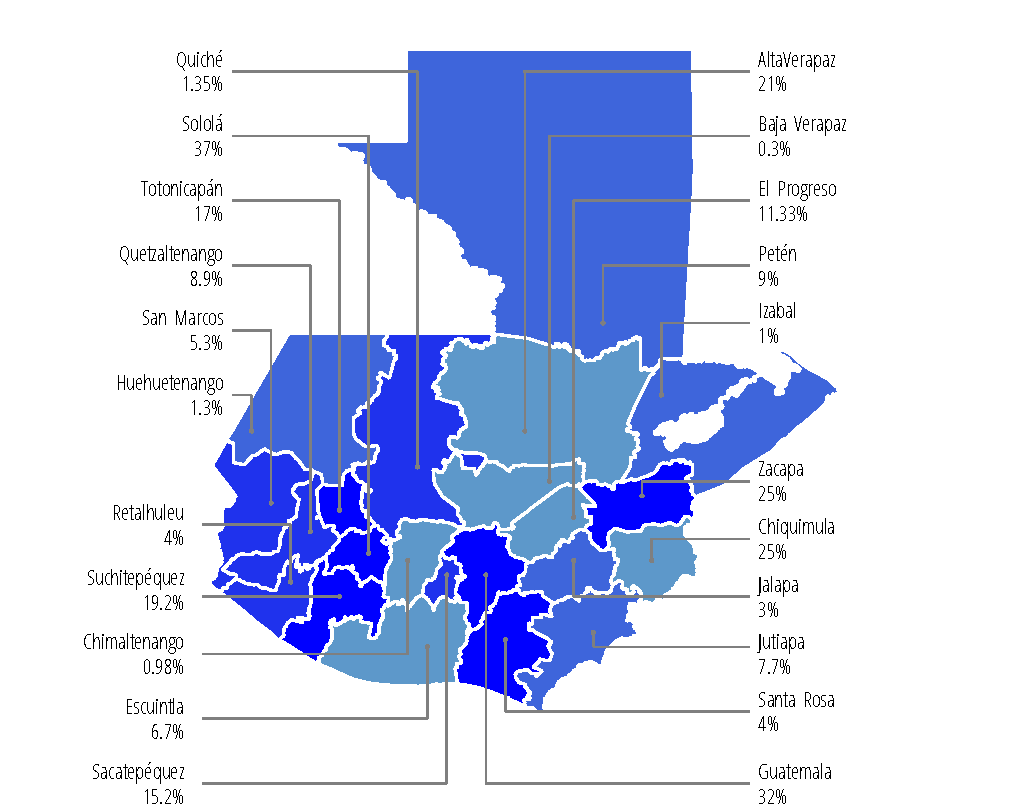
\includegraphics[width=52\cuadri]{graficas/1_10.pdf}  }{Instituto Nacional de Estadística}



\cajita{Brecha de pobreza total}{\footnote{$FGT(\alpha)=$
		
		$ \frac{1}{N}\sum_{i=1}^N \left(1-\frac{x_i}{LPT}\right)^\alpha (x_i<LPT) $\\
		
		Con $\alpha=1$}  La brecha de pobreza, muestra la distancia promedio a la que se encuentra la población en pobreza, a la línea de pobreza total y extrema, respectivamente.  
	
	Entre 2000 y 2014, se observa una reducción de la brecha de pobreza, principalmente para el caso de la pobreza total. 
	Este indicado permite hacer una estimación del monto que sería necesario transferir a los hogares de escasos recursos, para poder salir de la pobreza.}{Brecha de la pobreza total}{República de Guatemala, serie histórica por Encovi,  en porcentaje}{\ \\[0mm]\begin{tikzpicture}[x=1pt,y=1pt]  % Created by tikzDevice version 0.9 on 2015-11-26 22:13:04
% !TEX encoding = UTF-8 Unicode
\definecolor{fillColor}{RGB}{255,255,255}
\path[use as bounding box,fill=fillColor,fill opacity=0.00] (0,0) rectangle (289.08,198.74);
\begin{scope}
\path[clip] (  0.00,  0.00) rectangle (289.08,198.74);

\path[] (  0.00,  0.00) rectangle (289.08,198.74);
\end{scope}
\begin{scope}
\path[clip] (  0.00,  0.00) rectangle (289.08,198.74);

\path[] (  1.64, 17.78) rectangle (280.54,191.48);

\path[] (  1.64, 22.56) --
	(280.54, 22.56);

\path[] (  1.64, 60.67) --
	(280.54, 60.67);

\path[] (  1.64, 98.77) --
	(280.54, 98.77);

\path[] (  1.64,136.88) --
	(280.54,136.88);

\path[] (  1.64,174.99) --
	(280.54,174.99);

\path[] (  1.64, 41.61) --
	(280.54, 41.61);

\path[] (  1.64, 79.72) --
	(280.54, 79.72);

\path[] (  1.64,117.83) --
	(280.54,117.83);

\path[] (  1.64,155.94) --
	(280.54,155.94);

\path[] ( 53.94, 17.78) --
	( 53.94,191.48);

\path[] (141.09, 17.78) --
	(141.09,191.48);

\path[] (228.25, 17.78) --
	(228.25,191.48);
\definecolor{drawColor}{RGB}{0,0,255}

\path[draw=drawColor,line width= 1.7pt,line join=round] ( 53.94,183.59) --
	(141.09, 62.11) --
	(228.25,156.25);
\definecolor{drawColor}{RGB}{0,0,0}

\node[text=drawColor,anchor=base,inner sep=0pt, outer sep=0pt, scale=  1.01] at ( 53.94,187.54) {22.7};

\node[text=drawColor,anchor=base,inner sep=0pt, outer sep=0pt, scale=  1.01] at (141.09, 50.24) {19.5};

\node[text=drawColor,anchor=base,inner sep=0pt, outer sep=0pt, scale=  1.01] at (228.25,160.21) {22.0};

\path[draw=drawColor,line width= 0.1pt,line join=round] (  1.64, 25.67) -- (280.54, 25.67);

\path[] (  1.64, 17.78) rectangle (280.54,191.48);
\end{scope}
\begin{scope}
\path[clip] (  0.00,  0.00) rectangle (289.08,198.74);

\path[] (  1.64, 17.78) --
	(  1.64,191.48);
\end{scope}
\begin{scope}
\path[clip] (  0.00,  0.00) rectangle (289.08,198.74);

\path[] (  0.00, 41.61) --
	(  1.64, 41.61);

\path[] (  0.00, 79.72) --
	(  1.64, 79.72);

\path[] (  0.00,117.83) --
	(  1.64,117.83);

\path[] (  0.00,155.94) --
	(  1.64,155.94);
\end{scope}
\begin{scope}
\path[clip] (  0.00,  0.00) rectangle (289.08,198.74);

\path[] (  1.64, 17.78) --
	(280.54, 17.78);
\end{scope}
\begin{scope}
\path[clip] (  0.00,  0.00) rectangle (289.08,198.74);

\path[] ( 53.94, 13.51) --
	( 53.94, 17.78);

\path[] (141.09, 13.51) --
	(141.09, 17.78);

\path[] (228.25, 13.51) --
	(228.25, 17.78);
\end{scope}
\begin{scope}
\path[clip] (  0.00,  0.00) rectangle (289.08,198.74);
\definecolor{drawColor}{RGB}{0,0,0}

\node[text=drawColor,anchor=base,inner sep=0pt, outer sep=0pt, scale=  1.00] at ( 53.94,  2.85) {2000};

\node[text=drawColor,anchor=base,inner sep=0pt, outer sep=0pt, scale=  1.00] at (141.09,  2.85) {2006};

\node[text=drawColor,anchor=base,inner sep=0pt, outer sep=0pt, scale=  1.00] at (228.25,  2.85) {2014};
\end{scope}
  \end{tikzpicture}}{Instituto Nacional de Estadística}



\cajita{Brecha de pobreza extrema}{\footnote{$FGT(\alpha)=$
		
		$ \frac{1}{N}\sum_{i=1}^N \left(1-\frac{x_i}{LPT}\right)^\alpha (x_i<LPT) $\\
		
		Con $\alpha=1$}  La brecha de pobreza, muestra la distancia promedio a la que se encuentra la población en pobreza, a la línea de pobreza total y extrema, respectivamente. 
	
	Entre 2000 y 2014, se observa una reducción de la brecha de pobreza, principalmente para el caso de la pobreza total. 
	Este indicado permite hacer una estimación del monto que sería necesario transferir a los hogares de escasos recursos, para poder salir de la pobreza.}{Brecha de la pobreza extrema}{República de Guatemala, serie histórica por Encovi,  en porcentaje}{\ \\[0mm]\begin{tikzpicture}[x=1pt,y=1pt]  % Created by tikzDevice version 0.9 on 2015-11-26 21:53:27
% !TEX encoding = UTF-8 Unicode
\definecolor{fillColor}{RGB}{255,255,255}
\path[use as bounding box,fill=fillColor,fill opacity=0.00] (0,0) rectangle (289.08,198.74);
\begin{scope}
\path[clip] (  0.00,  0.00) rectangle (289.08,198.74);

\path[] (  0.00,  0.00) rectangle (289.08,198.74);
\end{scope}
\begin{scope}
\path[clip] (  0.00,  0.00) rectangle (289.08,198.74);

\path[] (  0.02, 17.78) rectangle (280.54,191.48);

\path[] (  0.02, 45.79) --
	(280.54, 45.79);

\path[] (  0.02, 78.43) --
	(280.54, 78.43);

\path[] (  0.02,111.07) --
	(280.54,111.07);

\path[] (  0.02,143.71) --
	(280.54,143.71);

\path[] (  0.02,176.34) --
	(280.54,176.34);

\path[] (  0.02, 29.48) --
	(280.54, 29.48);

\path[] (  0.02, 62.11) --
	(280.54, 62.11);

\path[] (  0.02, 94.75) --
	(280.54, 94.75);

\path[] (  0.02,127.39) --
	(280.54,127.39);

\path[] (  0.02,160.02) --
	(280.54,160.02);

\path[] ( 40.10, 17.78) --
	( 40.10,191.48);

\path[] (106.89, 17.78) --
	(106.89,191.48);

\path[] (173.68, 17.78) --
	(173.68,191.48);

\path[] (240.47, 17.78) --
	(240.47,191.48);
\definecolor{drawColor}{RGB}{0,0,255}

\path[draw=drawColor,line width= 1.7pt,line join=round] ( 40.10,183.59) --
	(106.89,172.55) --
	(173.68,150.57) --
	(240.47, 62.11);
\definecolor{drawColor}{RGB}{0,0,0}

\node[text=drawColor,anchor=base,inner sep=0pt, outer sep=0pt, scale=  1.01] at ( 40.10,187.54) {3.7};

\node[text=drawColor,anchor=base west,inner sep=0pt, outer sep=0pt, scale=  1.01] at (106.89,176.51) {3.4};

\node[text=drawColor,anchor=base west,inner sep=0pt, outer sep=0pt, scale=  1.01] at (173.68,154.53) {2.7};

\node[text=drawColor,anchor=base,inner sep=0pt, outer sep=0pt, scale=  1.01] at (240.47, 50.24) {0.0};

\path[draw=drawColor,line width= 0.1pt,line join=round] (  0.02, 25.67) -- (280.54, 25.67);

\path[] (  0.02, 17.78) rectangle (280.54,191.48);
\end{scope}
\begin{scope}
\path[clip] (  0.00,  0.00) rectangle (289.08,198.74);

\path[] (  0.02, 17.78) --
	(  0.02,191.48);
\end{scope}
\begin{scope}
\path[clip] (  0.00,  0.00) rectangle (289.08,198.74);

\path[] (  0.00, 29.48) --
	(  0.02, 29.48);

\path[] (  0.00, 62.11) --
	(  0.02, 62.11);

\path[] (  0.00, 94.75) --
	(  0.02, 94.75);

\path[] (  0.00,127.39) --
	(  0.02,127.39);

\path[] (  0.00,160.02) --
	(  0.02,160.02);
\end{scope}
\begin{scope}
\path[clip] (  0.00,  0.00) rectangle (289.08,198.74);

\path[] (  0.02, 17.78) --
	(280.54, 17.78);
\end{scope}
\begin{scope}
\path[clip] (  0.00,  0.00) rectangle (289.08,198.74);

\path[] ( 40.10, 13.51) --
	( 40.10, 17.78);

\path[] (106.89, 13.51) --
	(106.89, 17.78);

\path[] (173.68, 13.51) --
	(173.68, 17.78);

\path[] (240.47, 13.51) --
	(240.47, 17.78);
\end{scope}
\begin{scope}
\path[clip] (  0.00,  0.00) rectangle (289.08,198.74);
\definecolor{drawColor}{RGB}{0,0,0}

\node[text=drawColor,anchor=base,inner sep=0pt, outer sep=0pt, scale=  1.00] at ( 40.10,  2.85) {2000};

\node[text=drawColor,anchor=base,inner sep=0pt, outer sep=0pt, scale=  1.00] at (106.89,  2.85) {2006};

\node[text=drawColor,anchor=base,inner sep=0pt, outer sep=0pt, scale=  1.00] at (173.68,  2.85) {2011};

\node[text=drawColor,anchor=base,inner sep=0pt, outer sep=0pt, scale=  1.00] at (240.47,  2.85) {2014};
\end{scope}
  \end{tikzpicture}}{Instituto Nacional de Estadística}




\cajota{Brecha de la pobreza en los departamentos}{0}{Brecha de la pobreza total}{Por departamento, año 2014, en porcentaje}{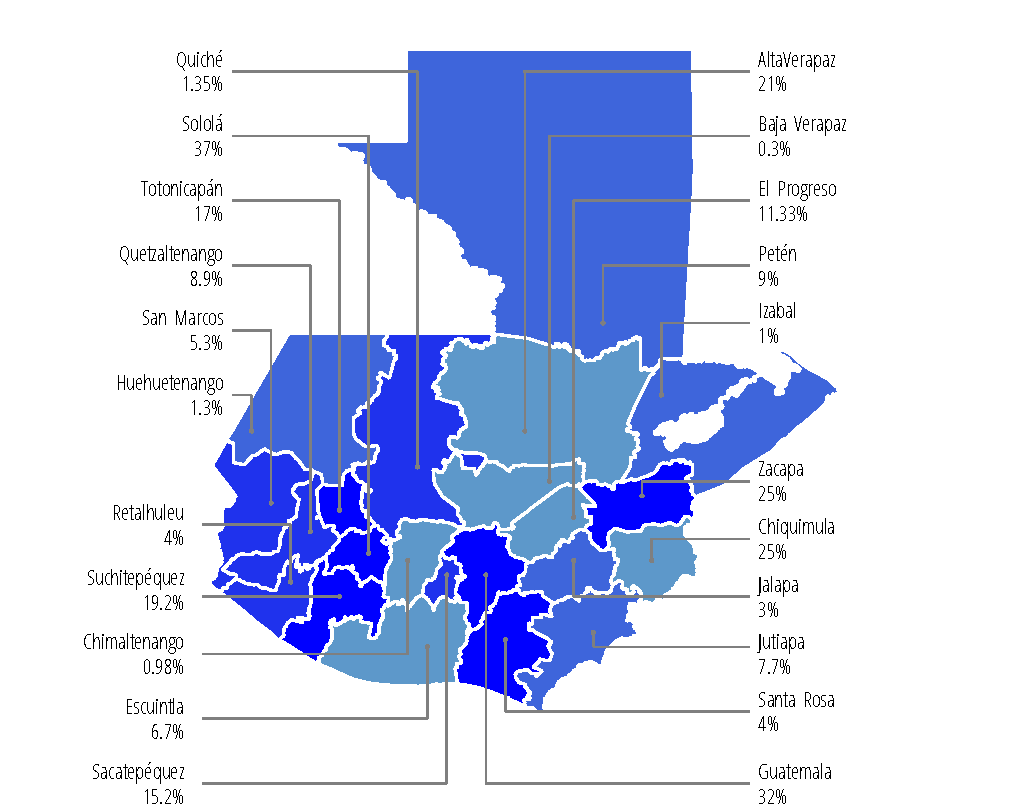
\includegraphics[width=52\cuadri]{graficas/1_13.pdf}  }{Instituto Nacional de Estadística}



\cajita{Severidad de la pobreza}{\footnote{$FGT(\alpha)=$
		
		$ \frac{1}{N}\sum_{i=1}^N \left(1-\frac{x_i}{LPT}\right)^\alpha (x_i<LPT) $\\
		
		Con $\alpha=2$}  El índice de severidad, es un índice compuesto que incorpora los tres elementos de la pobreza: incidencia, brecha y desigualdad. 
	
	En la grafía se puede observar que la severidad de la pobreza, se ha reducido en este período  de 11.7\% en 2000 a \% en 2014. }{Severidad de la pobreza total}{República de Guatemala, serie histórica por Encovi, en porcentaje}{\ \\[0mm]\begin{tikzpicture}[x=1pt,y=1pt]  % Created by tikzDevice version 0.9 on 2015-11-26 22:20:46
% !TEX encoding = UTF-8 Unicode
\definecolor{fillColor}{RGB}{255,255,255}
\path[use as bounding box,fill=fillColor,fill opacity=0.00] (0,0) rectangle (289.08,198.74);
\begin{scope}
\path[clip] (  0.00,  0.00) rectangle (289.08,198.74);

\path[] (  0.00,  0.00) rectangle (289.08,198.74);
\end{scope}
\begin{scope}
\path[clip] (  0.00,  0.00) rectangle (289.08,198.74);

\path[] (  1.64, 17.78) rectangle (280.54,191.48);

\path[] (  1.64, 59.45) --
	(280.54, 59.45);

\path[] (  1.64,114.75) --
	(280.54,114.75);

\path[] (  1.64,170.04) --
	(280.54,170.04);

\path[] (  1.64, 31.81) --
	(280.54, 31.81);

\path[] (  1.64, 87.10) --
	(280.54, 87.10);

\path[] (  1.64,142.39) --
	(280.54,142.39);

\path[] ( 53.94, 17.78) --
	( 53.94,191.48);

\path[] (141.09, 17.78) --
	(141.09,191.48);

\path[] (228.25, 17.78) --
	(228.25,191.48);
\definecolor{drawColor}{RGB}{0,0,255}

\path[draw=drawColor,line width= 1.7pt,line join=round] ( 53.94,183.59) --
	(141.09, 62.11) --
	(228.25,120.91);
\definecolor{drawColor}{RGB}{0,0,0}

\node[text=drawColor,anchor=base,inner sep=0pt, outer sep=0pt, scale=  1.01] at ( 53.94,187.54) {11.7};

\node[text=drawColor,anchor=base,inner sep=0pt, outer sep=0pt, scale=  1.01] at (141.09, 50.24) {9.5};

\node[text=drawColor,anchor=base,inner sep=0pt, outer sep=0pt, scale=  1.01] at (228.25,124.87) {10.6};

\path[draw=drawColor,line width= 0.1pt,line join=round] (  1.64, 25.67) -- (280.54, 25.67);

\path[] (  1.64, 17.78) rectangle (280.54,191.48);
\end{scope}
\begin{scope}
\path[clip] (  0.00,  0.00) rectangle (289.08,198.74);

\path[] (  1.64, 17.78) --
	(  1.64,191.48);
\end{scope}
\begin{scope}
\path[clip] (  0.00,  0.00) rectangle (289.08,198.74);

\path[] (  0.00, 31.81) --
	(  1.64, 31.81);

\path[] (  0.00, 87.10) --
	(  1.64, 87.10);

\path[] (  0.00,142.39) --
	(  1.64,142.39);
\end{scope}
\begin{scope}
\path[clip] (  0.00,  0.00) rectangle (289.08,198.74);

\path[] (  1.64, 17.78) --
	(280.54, 17.78);
\end{scope}
\begin{scope}
\path[clip] (  0.00,  0.00) rectangle (289.08,198.74);

\path[] ( 53.94, 13.51) --
	( 53.94, 17.78);

\path[] (141.09, 13.51) --
	(141.09, 17.78);

\path[] (228.25, 13.51) --
	(228.25, 17.78);
\end{scope}
\begin{scope}
\path[clip] (  0.00,  0.00) rectangle (289.08,198.74);
\definecolor{drawColor}{RGB}{0,0,0}

\node[text=drawColor,anchor=base,inner sep=0pt, outer sep=0pt, scale=  1.00] at ( 53.94,  2.85) {2000};

\node[text=drawColor,anchor=base,inner sep=0pt, outer sep=0pt, scale=  1.00] at (141.09,  2.85) {2006};

\node[text=drawColor,anchor=base,inner sep=0pt, outer sep=0pt, scale=  1.00] at (228.25,  2.85) {2014};
\end{scope}
  \end{tikzpicture}}{}



\cajota{Severidad de la pobreza en los departamentos}{ }{Severidad de la pobreza total}{Por departamento, año 2014, en porcentaje}{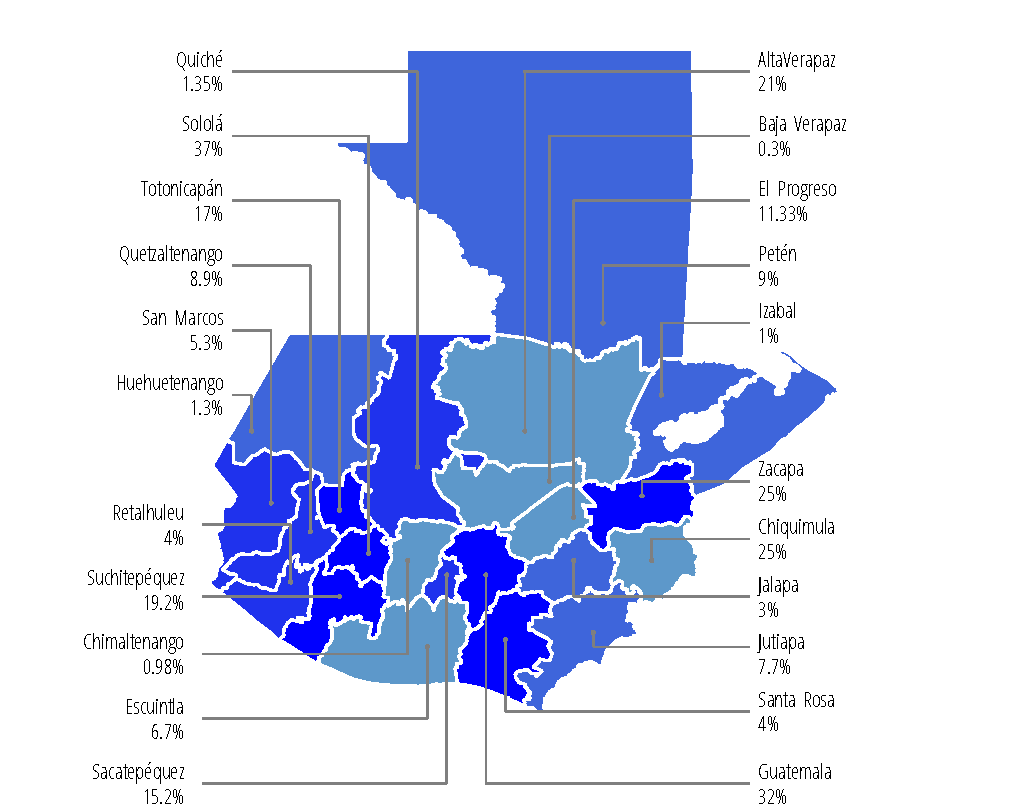
\includegraphics[width=52\cuadri]{graficas/1_15.pdf}  }{ }
